\label{sec:relatedworks}
\subsection{Генеративные состязательные сети}

Генеративные состязательные сети (\emph{Generative adversarial network}, сокр., \emph{GAN})  это семейство генеративных моделей, разработанное Яном Гудфеллоу в 2014 году \cite{goodfellow2014generative}.  Они формулируют процесс ~обучения (подгонки, fitting) генеративной модели~ в виде антагонистической игры между двумя игроками: \emph{генератором} и \emph{дискриминатором}.

% набор синтетических данных. Эти данные represent выучиваемое распределение q(x) 
% пытаясь аппроксимировать обучающую выборку, полученную из распределения реальных данных $q_{data}(x)$
Генератор $G$ представляет собой глубокую нейронную сеть, задающую отбражение из латентного пространства $Z$ в пространство данных $\mathcal X$.
Принимая на вход случайные вектора из некоторого заданного распределения $p(z)$ в $Z$, он производит набор синтетических данных, пытаясь аппроксимировать распределение обучающей выборки $q_{data}(x)$.

% распределения реальных данных $q_{data}(x)$ ?== распределение обучающей выборки $q_{data}(x)$
Дискриминатор $D$ представляет собой глубокую нейронную сеть, задающую отбражение из пространства данных $\mathcal X$ в $\mathbb R$. Получив на вход некоторый элемент из пространства $\mathcal X$, дискриминатор ~возвращает~(характеризует) вероятность того, что он был получен из распределения реальных данных $q_{data}(x)$, а не сгенерирован генератором $G$.

\begin{figure}[h]
\begin{center}
    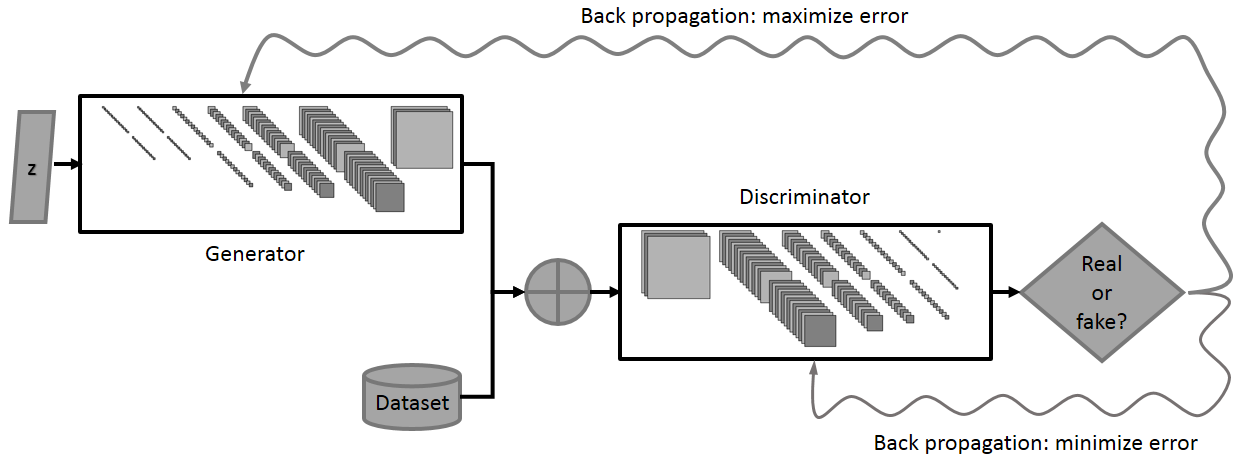
\includegraphics[width=0.9\textwidth]{gan}
    \caption{Архитектура генеративной состязательной сети (написать откуда взял)}
    \label{fig:subim11}
\end{center}
\end{figure}

Роль дискриминатора состоит в том, чтобы как можно более точно отличать синтетические данные, полученные генератором, от реальных данный, взятых из обучающей выборки, в то время как генератор пытается обмануть дискриминатор путем генерирования синтетических данных, как можно более похожих на реальные.
% Following the more general formulation introduced in [39], the GAN learning problem entails finding the minimax with respect to the pair(G,D) (i.e., the Nash equilibrium), of the value function defined as
Процесс совместного конкурентного обучения продолжается вплоть до достижения парой $(G, D)$ <<седловой точки>> (т.е. равновесия по Нэшу) \cite{goodfellow2017nips} функции выигрыша
$$
\min_{G} \max_{D} V(G, D) = \mathop{\mathbb{E}}_{x \sim q_{data}(x)} [\log D(x)] + \mathop{\mathbb{E}}_{z \sim p(z)} [\log (1 - D(G(z)))] ,
$$
в которой генератор способен генерировать данные, неотличимые дискриминатором от реальных.

\subsection{Генеративные нейронные сети для генерации лиц}
% Нужно тут водинисто вводить в задачу генерации изображений, не перечислять решения, а рассказывать как кокой-то таймлаин.

При решении задачи генерации изображений (в.т.ч. изображений лиц), в качестве дискриминатора используется сверточная нейронная сеть [VGG / conv ?], а в качестве генератора --- сверточная нейронная сеть со слоями транспонированной свертки [DCGAN].
Пространство данных $\mathcal X$ в данном случае предстваляет собой пространство изображений, каждый элемент которого обладает некоторым набором семантических признаков, например в случае лиц --- положение головы, пол, возраст.
%Тут нужно сказать про латентное пространство, и рас уж мы заговорили про семантические признаки, то curvature и disentanglement.


\paragraph{BigGAN.}
% Вначале сказать "BigGAN ...", а потом то какую проблему он решает
Генерация изображений высокого разрешения довольно долго была трудной(непосильной) задачей для GAN-ов. Она требует генеративной модели с большим количеством параметров, что, в случае GAN-ов, сказывается на стабильности обучения [че то типа Why GANs are hard to train].

% ... разработанная компанией DeepMind.
(Генеративная состязательная сеть) BigGAN \cite{bigGAN} являлась ?первым шагом к решению данной проблемы. Эта сеть спроектирована с целью масштабирования архитектуры для генерации изображений высокого разрешения.
Она внесла ряд модификаций в стандартную архитектуру генеративных состязательных сетей (и процесс генерации), таких как self-attention слой, спектральная нормализация весов (, Truncation Trick). Это позволило увеличить количество весов моддели в 2 раза и добиться качественной генерации изображений с разрешением до $512\times512$ на самых разнообразных классах изображений.
% ! Это не имеет особого отношения к теме работы, поэтому не надо !
% https://machinelearningmastery.com/a-gentle-introduction-to-the-biggan/
% https://arxiv.org/abs/1805.08318  таких как self-attention слой
% https://arxiv.org/abs/1802.05957  спектральная нормализация весов


\paragraph{StyleGAN.}
StyleGAN \cite{StyleGAN} – это генеративная состязательная сеть, архитектура которой разрабатывалась специально с целью генерации реалистичных изображений лиц.
Одной из сложностей генерации изображений является кривизна, или запутенность (\emph{entanglement}), латентного пространства. 
Входное латентное пространство $\mathcal Z$ должно подстраиваться под вероятносное распределение тренировочных данных, а потому любые сдвиги/неточности, например отсутствие в тренировочных данных комбинации нескольких признаков (Рис. \ref{fig:stylegan-mapping}), приводят к искажениям.
% Это либо здесь написать, либо расписать в изображениии: This forces the mapping from Z to image features to become curved ...
% про то что метрики(линейные расстояния) в латентном пространстве не соответствуют расстояниям в пространстве данных.
В результате латентное пространство (приходится рассматривать) не как линейное евклидово пространство, а как искривленное пространство \cite{arvanitidis2018oddity}.
% In general, latent space distances lack physical units (making them difficult to interpret) and are sensitive to specifics of the underlying neural nets. It is therefore more robust to consider infinitesimal distances along the data manifold in the input space... Mathematically,  the  latent  space  should  not then  be  seen as a linear Euclidean space,  but rather as a curved space

%https://neurohive.io/ru/papers/stylegan-open-source/   
StyleGAN предлагает альтернативную архитектуру генератора, которая основывается на идеях из style transfer. 
Синтез изображения начинается с фиксированного входного вектора, а информация о латентном представлениии последовательно встраивается в каждый слой генератора, начиная с первых слоев генератора с пространственной размерностью $4\times4$ и заканчивая последними слоями с размерностью $1024\times1024$.
Это позволяет контролировать силу проявления различных семантических признаков изображения на разных ?масштабах, от грубых признаков до тонких деталей.
%Our generator starts from  a  learned  constant  input  and adjusts  the  “style”  of the  image  at  each  convolution  layer  based  on  the  latent code,  therefore  directly  controlling  the  strength  of  image features at different scales. 
В сочитании с встраивании шума напрямую в слои сети, такая архитектура позволяет отделить высокоуровневые атрибуты изображения (положения лица, личность человека) от случайных вариационных факторов (волосы, веснушки и т.п.).
%Combined with noise injected directly into the network, this architectural change leads to automatic, unsupervised separation of high-level attributes(e.g., pose, identity) from stochastic variation (e.g., freckles,  hair)  in  the  generated  images,  and enables  intuitive scale-specific mixing and interpolation operations.
% !Сказать, про W+ (или сказать про это потом)

% !Перенести это наверх, до архитектуры
Одной из ключевых особенностей архитекуры StyleGAN является наличие промежуточного латентного пространства $\mathcal W$. Во время обучения StyleGAN выучивает нелинейное преобразование $f: \mathcal Z \mapsto \mathcal W$, что позволяет избавиться от ограничений, накладываемых вероятносным распределением тренировочных данных, и получить более линейное латентное пространство.

\emph{Нужно поправить изображение и решить, насколько дословно расписывать пример}

\begin{figure}[h]
\begin{center}
    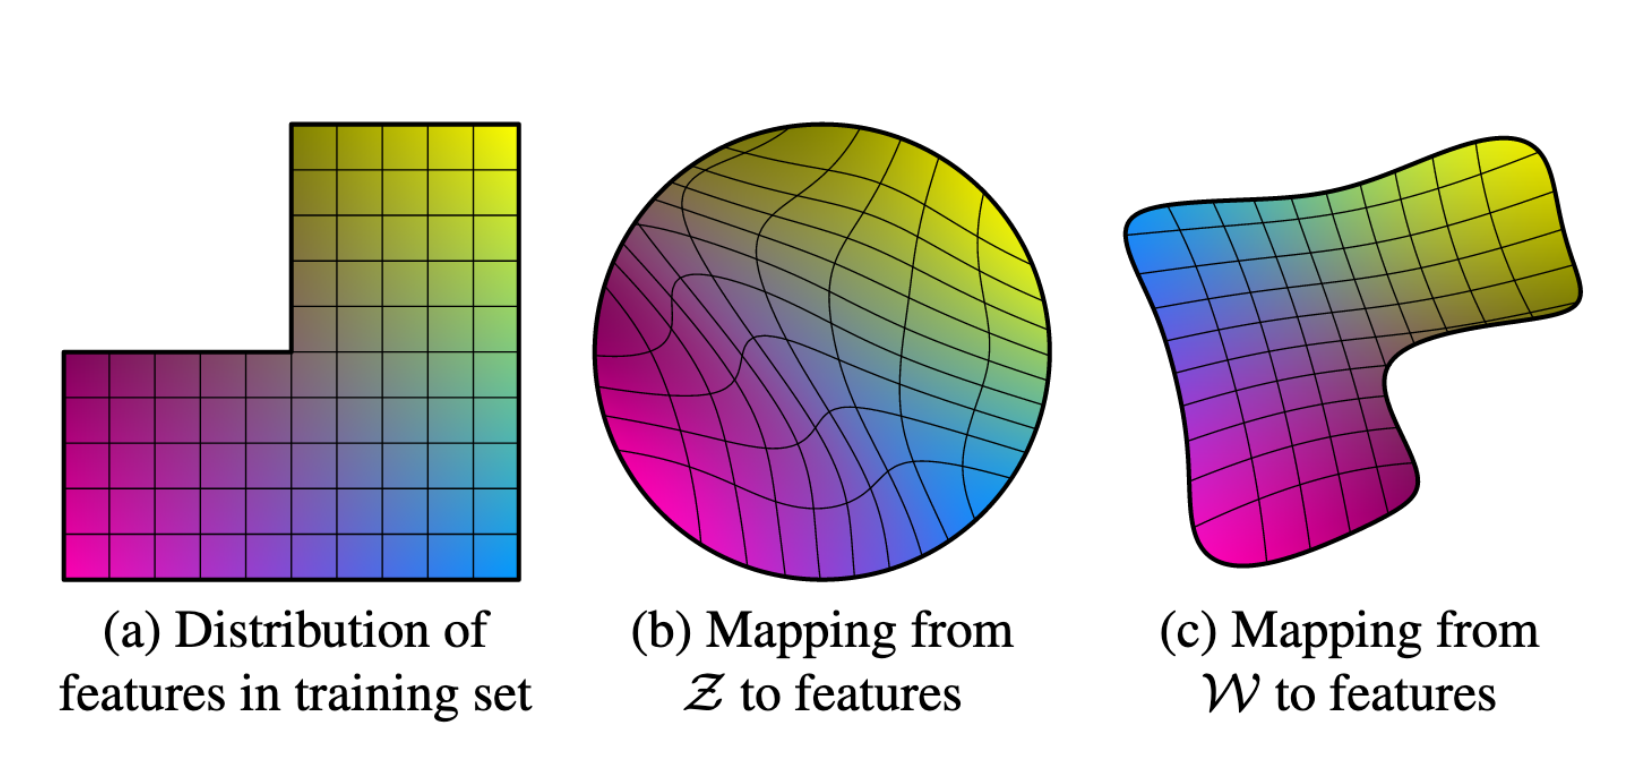
\includegraphics[width=0.7\textwidth]{stylegan_mapping}
    \caption{Иллюстрация действия промежуточного латентного пространства на примере двух факторов вариации. Изображение взято из \cite{StyleGAN}.}
    \label{fig:stylegan-mapping}
\end{center}
\end{figure}
% Illustrative example with two factors of variation (image features, e.g., masculinity and hair length).  (a) An example training set where some combination (e.g., long haired males) is missing. (b) This forces the mapping from Z to image features to become curved so that the forbidden combination disappears in Z to prevent the sampling of invalid combinations.  (c) The learned mapping from Z to W is able to “undo” much of the warping.


\paragraph{ALAE.}
%https://arxiv.org/pdf/1511.05644.pdf  Adversarial Autoencoders
%We designed an AE architecture where we allow the latent distribution to be learned from data to address entanglement (A). The output data distribution is learned with an adversarial strategy (B). Finally, to implement (A) and (B) we impose the AE reciprocity in the latent space (C).

% декомпозируем генератор и дискриминатор ... - но это не очень понятно
ALAE \cite{ALAE} – это генеративная нейронная сеть, которая совмещает в себе особенности генеративных состязательных сетей и вариационных автоэнкодеров [].

Она модифицирует стандартную архитектуру генеративных состязательных сетей путем добавления \emph{перед} генератором и \emph{перед} дискриминатором некоторых выучваемых отображений в промежуточное латентное пространство.
% наложение на промежуточное латентное пространство ограничения о взаимной близости представлений дает возможность выучить latent distribution с помощъю autoencoder стратегии, и data distribution с помощью состязательной стратегии.
Из-за этого он жертвует качеством генерации, но дополнительно выучивает обратное отображение в латентное пространство сети.


\subsection{Методы отображения изображений в латентное пространство сети}
% TODO выровнять алгоритмы/методы/подходы
Для работы с реальными изображениями генеративным состязательным сетям требуется обратное отображение, позволяющее по входному изображению получить соответствующий ему латентный вектор. Классическая архитектура генеративных состязательных сетей не задает такого отображения напрямую, а потому для его получения используются (различные приближения).

%% \subsubsection{Обучение дополнительного энкодера}
Одним из самых распространенных подходов \cite{donahue2016adversarial} является обучение энкодера --- дополнительной нейронной сеть, которая будет отображать входное изображение в латентное пространство заданной генеративной состязательной сети. 
% Такой энкодер может встраиваться в процесс обучения GAN-а, и обучаться совместно с генератором и дескриминатором, или же являться отдельной моделью, обучающейся при фиксированном GAN-е.

%% \subsubsection{Латентная оптимизация}
% Здесь сказать про то что ГАН дифференциирум по входам, потому что композиция линейных и активаций.
Другие подходы \cite{perarnau2016invertible} напрямую оптимизируют латентный вектор, минимизируя некоторую заданную функцию потерь реконструкции.
Генератор генеративной состязательной сети является композицией линейных слоев и функций активации, а потому при использовании гладких функций акнивации также является гладким отображением.
Это позволяет применить градиентный спуск и метод обратного распространения ошибки для нахождения латентного вектора, минимизирующего заданную функцию потерь реконструкции.

%То, что в качестве функции потерь используется не L2 а perceptual loss (или в архитектуре/реализации).

Несмотря на гибкость GAN-ов, они ограницены распределением тренировочных данных. Из-за искривления они не могут генерировать комбинации признаков, которых не было в тренировочных данных(, а также получают плохие результаты когда сэмпл далеко от тренировочного распределения <-- ото может ниже). [What GANs cannot generate, Cheese theorem]. 

% ! TODO:
(Латентная оптимизация в Z застрянет в локальном минимуме.
StyleGAN позволяет производить латентную оптимизацию в W и улучшить сходимость.
Более того, архитектура StyleGAN позволяет в каждый из 18 слоев встраивать отдельное латентное представление, и тем самым оптимизировать в расширенном пространстве W+ и получить с помощью такой оптимизации изображение, которое невозможно было бы получить в обычной генерации [Image2StyleGAN].)


\subsection{Методы выделения семантик изображения в латентном пространстве сети}
Идея манипулирования латентным вектором в латентном пространстве генеративной состязательной сети основана на наблюдении о том, что к латентным векторам применима векторная арифметика \cite{radford2015unsupervised}.
% Из этого возникает идея нахождения преобразований в латентном пространстве, которые соответствовали бы изменениям семантических признаков на генерируемом изображениии.

Другой подход \cite{hrknen2020ganspace} использует метод главных компонент для уменьшения размерности латентного пространства и выделения наиболее важных направлений. Дальнейший визуальный/качественный анализ полученных направлений показывает, что они соответствуют значимым изменениям в изображении.

Один из существующих подходов \cite{shen2020interfacegan} выдвигает предположение о линейности латентного пространства, и исследует его с целью нахождения векторов, соответствующих определенным заданным изменениям в признаках изображения.


